\chapter{Introduction\label{cha:introduction}}
%% \ifdraft only shows the text in the first argument if you are in draft mode.
%% These directions will disappear in other modes.
%\ifdraft{State the objectives of the exercise. Ask yourself:
%  \underline{Why} did I design/create the item? What did I aim to
%  achieve? What is the problem I am trying to solve?  How is my
%  solution interesting or novel?}{}
%
%\section{Background}
%\ifdraft{Provide background about the subject matter (e.g. How was morse code
%developed?  How is it used today?). 
%This is a place where there are usually many citations.
%It is suspicious when there is not.
%Include the purpose of the different equipment and your design intent. 
%Include references to relevant scientific/technical work and books.
%What other examples of similar designs exist?
%How is your approach distinctive?
%
%If you have specifications or related standards, these must be
%described and cited also.  As an example, you might cite the specific
%RoboSub competition website (and documents) if working on the lighting system for an AUV\cite{guls2016auvlight}
%
%%% Glossary is broken, do not use --foley
%% \gls{auv}\footnote{Autonomous Undersea Vehicle}.


%%%%% -------------------------------------------------------- %%%%%%%
%% \ifdraft only shows the text in the first argument if you are in draft mode.
%% These directions will disappear in other modes.
%% \textit{State the objectives of the exercise. Ask yourself:}
%%  \underline{Why} \textit{did I design/create the item? What did I aim to
%%  achieve? What is the problem I am trying to solve?  How is my
%%  solution interesting or novel}? \\
\ifdraft{
 \label{Chapter: 1}
 Electricity is one of the foundation of everyday life. Electricity is a widely used commodity in advanced countries and is being set up in third world countries.    A quote from the Russian politician Boris Yeltsin is "We don't appreciate what we have until it's gone"\footnote{\url{https://www.brainyquote.com/quotes/quotes/b/borisyelts371415.html}}. The quote has meaning for multiple meanings and one certainly holds true for electricity. When it is operational everybody is happy but when it is non-operational, nobody is happy. There are workplaces that are very dependent on electricity for example hospitals, factories, emergency services. The loss of electricity can lead to money loss for the consumer if the power is not consistent or working for a long period time. }{}
 

 
\section{Power system}\label{Chapter: 1-Power System}  
 \ifdraft{
The set up for the basic power station is as follows
\begin{enumerate}
\itemsep0em 
\item Electricity Generation
\item Step Up Transformer
\item Transmission Line
\item Step Down Transformer
\item Consumer
\end{enumerate}
\newpage
The basic set up for a power systems can be seen in figure \ref{Fig: Basic Structure of the Electric System}\footnote{\url{http://www2.econ.iastate.edu/classes/econ458/tesfatsion/Home458Team.htm}}.
 \begin{figure}[h!]
 \center
 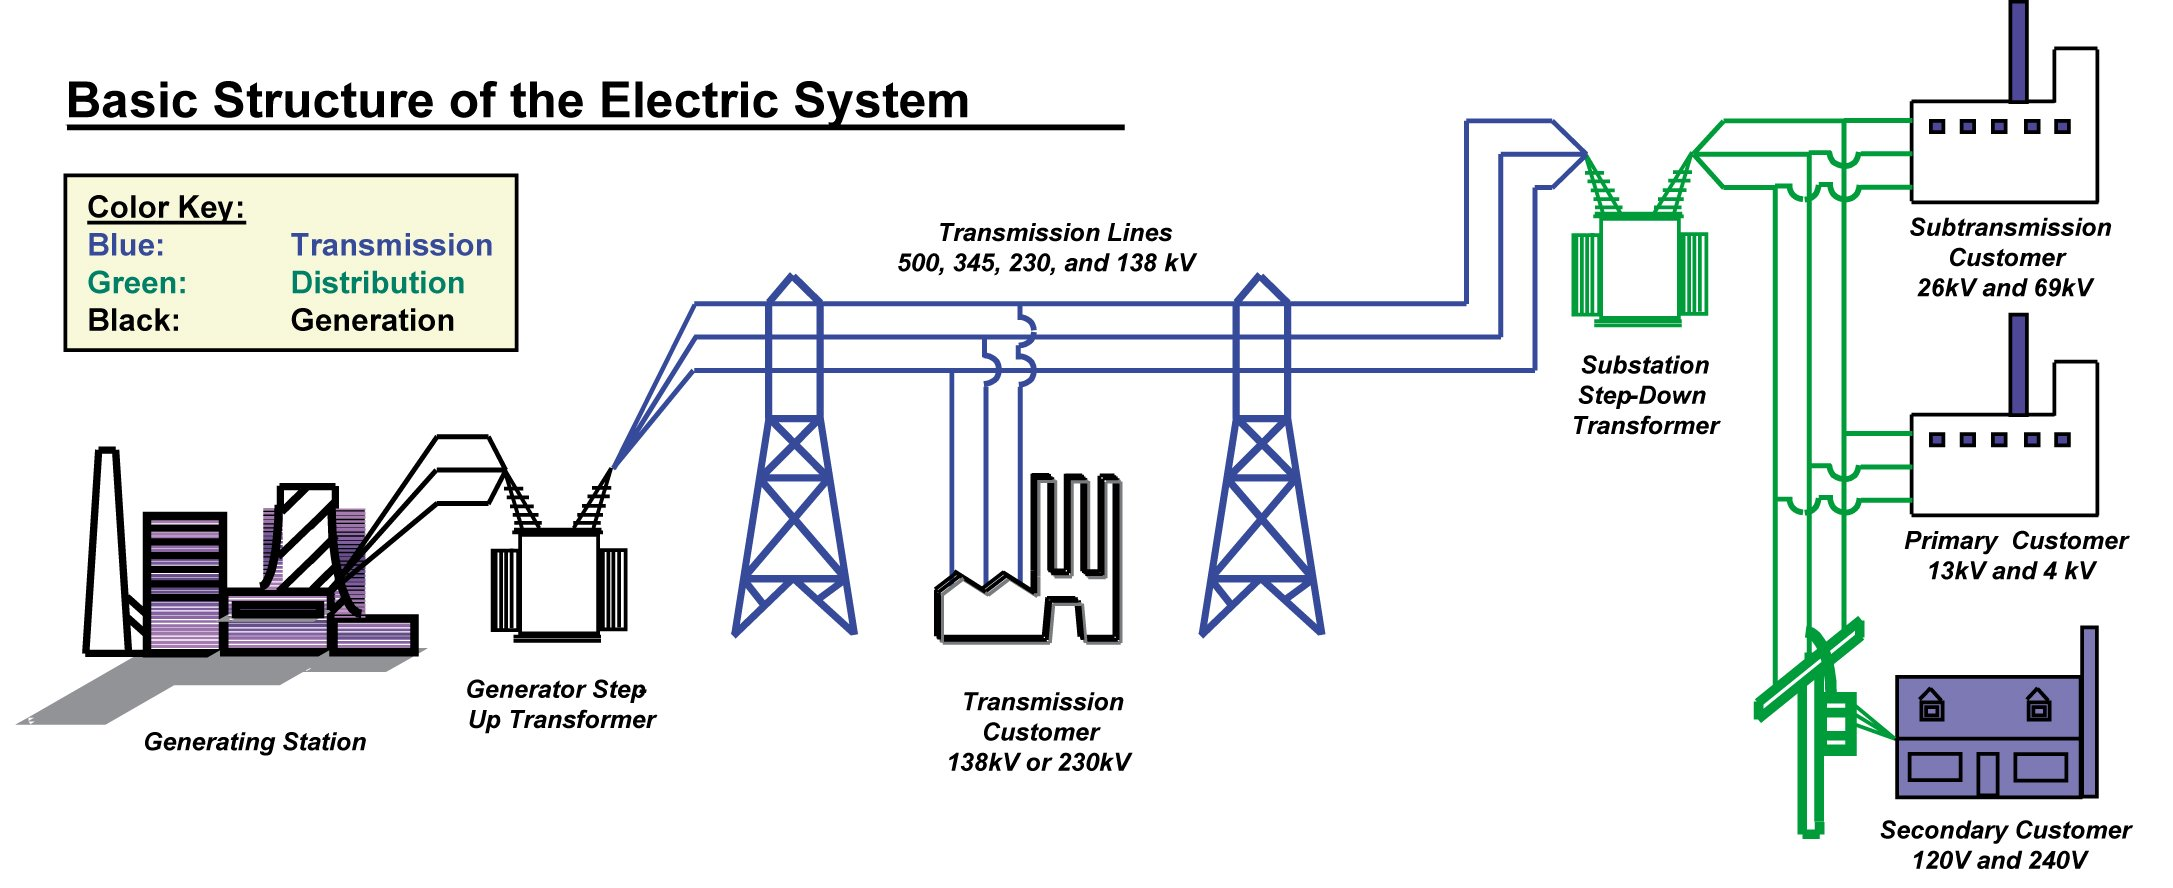
\includegraphics[scale=0.15]{graphics/ElectricPowerSystem.jpg}
 \caption{Structure of a Power System}
 \label{Fig: Basic Structure of the Electric System}
 \end{figure}\\
The first step is the power generation that can be varied from oil, hydro, gas, nuclear, coal, wind, solar and other renewable sources as a single unit or a combination of multiple units. The World Eenergy Council\footnote{\url{https://www.worldenergy.org/wp-content/uploads/2016/10/World-Energy-Resources-Full-report-2016.10.03.pdf}} shows the usages of these electricity generations from the past 15 years which are changing as can be seen in figure \ref{Fig: Electricity generation from 2005 to 2015}\footnote{\url{https://www.worldenergy.org/wp-content/uploads/2016/10/World-Energy-Resources-Full-report-2016.10.03.pdf}}.
 \begin{figure}[h!] 
  \center
  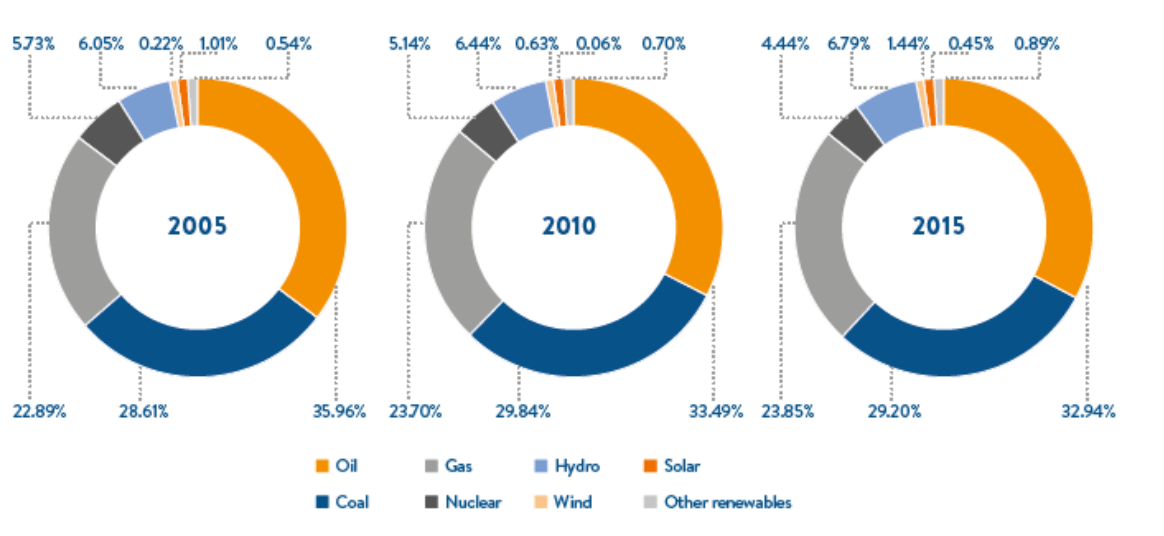
\includegraphics[scale=0.5]{graphics/PrimaryEnergyConsumption.PNG}
  \caption{Electricity generation from 2005 to 2015}
  \label{Fig: Electricity generation from 2005 to 2015}
  \end{figure}\\
  Step 2,3 and 4 there are two kind of transformers that are the step up and step down and the transmission line between them.  Since in many instances the power generation is not in close proximity to where the consumer, then the electricity needs to be sent to the consumer. \newpage
 The voltage needs to be scaled up to be able to go through the transmission line, where the loss of voltage is inconsequential. When the distance to the consumer is reached than the voltage needs to be scaled down to be in working conditions. 
The consumer can also be directly connected with the transmission
 line for example factories with heavy electrical consumption. The regular consumer needs the voltage to be between  230 to 250 V in Europe and 110 V in America \footnote{\url{http://engineering.electrical-equipment.org/electrical-distribution/importance-of-voltage-criteria-for-consumer-distribution-system.html}}. The electricity might have gone through multiples of transformers until it has reached its final destination.
 
  }{}
  \section{Transformer} \label{Chapter: 1-Transformer} 
   \ifdraft{
  The transformer is one of the main units in a power structure, since they enable the power companies to send the voltage from the power generators over long distances and be usable for the consumer. The transformer is the most valuable unit and the the price and size of the transformer varies by manufacturer and some can cost millions of dollars \cite{LARGE-POWER-TRANSFORMERS-AND-THE-U.S.ELECTRIC-GRID}.  The workability of the transformer is crucial and there-fore the maintenance and protection is of high importance.  The failure of the transformer can be divided into two groups 
  \begin{enumerate}
  \item Internal
  \item External
  \end{enumerate}
It will be in more detail in next chapter about what failures are in each group.
 
  }{}
  \newpage
  \subsection{Working of transformer} \label{Chapter: 1-Working of transformer}
  \ifdraft{
  The workings of a power transformer is that two windings are on a single core to get magnetic coupling see fig \ref{Fig: Ideal transformer with two winding on a single core}\footnote{\url{https://en.wikipedia.org/wiki/Transformer}}
  \begin{figure}[h!]
  \center
  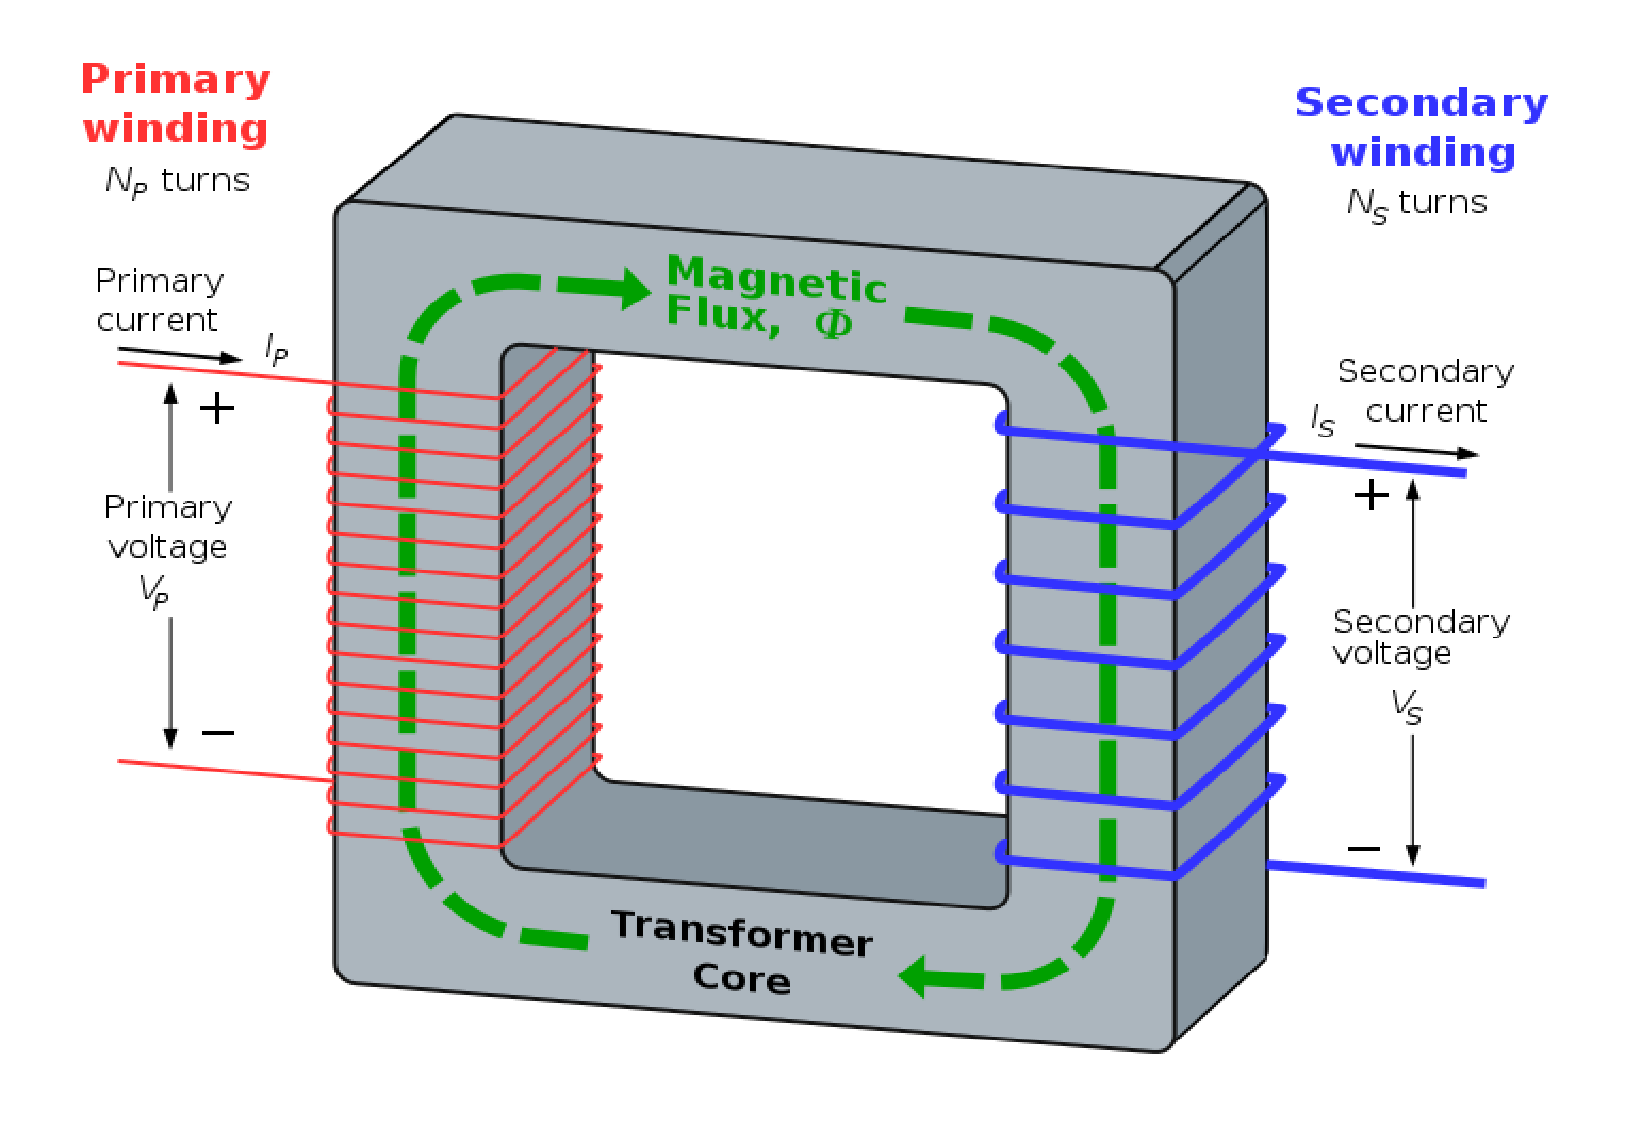
\includegraphics[scale=0.4]{graphics/763px-Transformer3d_col3.pdf}
  \caption{Ideal transformer with two winding on a single core}
  \label{Fig: Ideal transformer with two winding on a single core}
  \end{figure}\\
The windings are split into the primary (N$_p$) where the primary voltage (V$_p$) and current (I$_p$) goes through that produces magnetic field. Secondary windings (N$_s$) gets the magnetic field and creates electric current (I$_s$) and voltages (V$_s$) .  The idealized model for the transformer is the following\cite{Power_Electronics}:
\begin{equation}
\begin{split}
\dfrac{V_p}{V_s} = \dfrac{N_p}{N_s} \\
\dfrac{I_p}{I_s} = \dfrac{N_s}{N_p}
\end{split}
\label{Math: Voltage, Current and Turns ratio}
\end{equation} 
  where the V$_p$ and V$_s$ are proportional to the number of windings  
in N$_p$ and N$_s$.  
  For a step up transformer then the windings would be $N_p < N_s$ and for a step down it would be other way around as the figure above shows how step down transformer windings would be.
  }{}
  \newpage
\section{Types of Transformers}
\ifdraft{
There are few types of transformers used in power systems and are the following\footnote{\url{https://www.slideshare.net/vasanthancore/different-types-of-transformers-used-in-generating-station}} 
\begin{itemize}
\item Generator Transformer (GT)
\item Station Transformer (ST)
\item Distribution Transformer (DT)
\item Unit Auxiliary Transformer (UAT)
\item Auxiliary Transformer (AT)
\item Instrument Transformer (IT)
\item Rectifier Transformer (RT)
\item Neutral Ground Transformer (NGT)
\end{itemize}
  The GT is used in generating stations to step up the voltage for the use of transmitting the voltage with the transmission lines in the power grid. GT reduces voltage losses when transmitting the voltage over long distances and take much space so they are usually installed outdoors.\\
  The ST is used for when the power plant is not generating power, to supply the auxiliary equipment necessary power to function in the power station.\\
  The DT is a step down transformer that is used to lower the voltage to the supplier need.  \\
 The UAT is connected to the generator terminals and provides power to the generator auxiliaries of that unit. There is one UAT for every generating unit in power generating station.  \\
  The AT is used to step down the voltage to the low voltage loads in a power station where the voltage is lower than 1KV.\\  
  The IT is used in AC systems for protection system in power systems where they are connected line that has very high voltage and currents and lower the values to a more workable value.  There are two types of IT and they are current transformer (CT) and potential transformer (PT). Where the CT steps down the current from HC to LC so low budget ammeter can be used to measure the current and the current is safer to work with. PT is used to step down the voltage from HV to LV so that a low rating voltmeter can be used to read the values, the value can be 110 - 120 V.  Using the CT and PT for measuring purposes in power stations lower the budget for measuring units.  Where they take the current and voltage levels from very high rating that can be life threatening to a much safer values and readable values.\footnote{\url{https://www.electrical4u.com/instrument-transformers/}}\footnote{\url{https://hubpages.com/technology/Differenet-Transformers-in-Power-Station}}\\
  The RT is a combinations of either diode or thyristors that are connected to the secondary side and change the AC to a DC. These transformer are used in industries where the supply of DC is significant for instance aluminium smelting factories where the furnaces need lot of power to operate.\footnote{\url{http://www.studyelectrical.com/2015/11/what-rectifier-transformers-operation-and-application.html}}\\ 
  The NGT is used for resistance ground protection from damaging fault currents with low resistance. These devices  are able to clear the fault within a few seconds and prevent the current to overheating on conductors.\footnote{\url{http://www.postglover.com/wp-content/uploads/downloads/2014/04/GT110-08_NGR_Trans.pdf}} 
    }
    
  \section{Objective of this thesis}
  \ifdraft{
  The object of this thesis is to research, build and make a monitoring and protection system for a three phase power transformer by using sensors and micro-controller (M-C). The M-C will read data from the sensors that will be placed on tested transformer.  The research will provide with that transformer failures happens to a transformer and what to look out for. There are optimal operating values for transformers but they depends on what kind and for what use it is for. If the values are not in the given optimal values the M-C will send an alarm and if needed cut off the power to the transformer before to much damage happens.  The data collected in the M-C is sent to a program that will display the information for a human operator.  The program will also allow the human operator to some control of the operation of the M-C.       
   }{}


%
%\section{Background}
%\ifdraft{Provide background about the subject matter (e.g. How was morse code
%developed?  How is it used today?). 
%This is a place where there are usually many citations.
%It is suspicious when there is not.
%Include the purpose of the different equipment and your design intent. 
%Include references to relevant scientific/technical work and books.
%What other examples of similar designs exist?
%How is your approach distinctive?



%% Notice that there is now information on the AUV in the Index and Acronyms.
%% It isn't in the \gls{glossary} because we didn't put it there.
%\index{AUV}
%}{}
%
%\section{Example Section}
%The test text ``Lorem Ipsum''\index{Lorem Ipsum} is from an ancient text from 45 B.C. \cite{cicero46deFinibus, lipsomwebsite}\\
%\lipsum[1-5]
%\subsection{Subsection}
%\lipsum[6-10]
%\subsubsection{SubSubsection}
%\lipsum[11-15]
%%%% Local Variables: 
%%%% mode: latex
%%%% TeX-master: "MSC-NAME-YEAR"
%%%% End: 
